\documentclass[a4paper]{article}

\usepackage[english]{babel}
\usepackage[utf8]{inputenc}
\usepackage{amsmath}
\usepackage{graphicx}
%\usepackage[colorinlistoftodos]{todonotes}

\title{GridPACK Validation Report on State Estimation}

\author{Yousu Chen}

\date{\today}

\begin{document}
\maketitle

This documentation has been prepared to validate the GridPACK state estimation
(SE) module. Because a commercial SE tool is not available to validate against,
the validation was conducted by comparing the SE outputs against  measurements
obtained from a powerflow solution. Using this strategy, the SE results are
expected to self-consistently match the poweflow solution. If the maximum
absolute difference between SE estimates and the measurements is smaller than
a preset tolerance, the SE application is considered to meet the validation
requirements.  

During the validation, three power systems, the IEEE 118-bus network, a
3,000-bus network, and a 20,000-bus network representing the Western Electricity
Coordinating Council (WECC), were used to represent small, medium, and large
systems. Power flow solutions for each test system are used as measurements.
The types of measurements include bus voltage magnitude ($V_M$), real power
injection ($P_I$), reactive power injection ($Q_I$), real power flow in both
directions ($P_{IJ}$ and $P_{JI}$), and reactive power flow in both directions
($Q_{IJ}$ and $Q_{JI}$). Table~\ref{tab:SE}  contains the details of
measurement type and the associated measurement deviation.

\begin{table} [h]
\centering
\begin{tabular}{l|r}
Type of measurements & Deviation \\\hline
$V_M$	& 0.015 \\
$P_I$	& 0.015 \\
$Q_I$	& 0.015 \\
$P_{IJ}$	& 0.01 \\
$P_{JI}$	& 0.01 \\
$Q_{IJ}$	& 0.01 \\
$Q_{JI}$	& 0.01

\end{tabular}
\caption{\label{tab:SE}Type of measurements and measurement deviations used in State Estimation Validation.}
\end{table}

The SE validation is based on comparing the maximum absolute differences
between measurements and SE estimates against SE tolerance. The histogram of
these differences for each test systems are provided below.


\newpage
\section{IEEE 118-bus test system}
\label{sec:118}

712 measurements based on the power flow solution were applied to the 118-bus
test system with a tolerance of $10^{-4}$.  The largest difference between SE
output and the power flow solution is $6.0*10^{-5}$, which is smaller than the
tolerance.  The histogram of the absolute differences between measurements and
estimates is shown in Figure  \ref{fig:118}.  Table \ref{tab:118} summarizes
the validation results.

\begin{figure}[h]
\centering
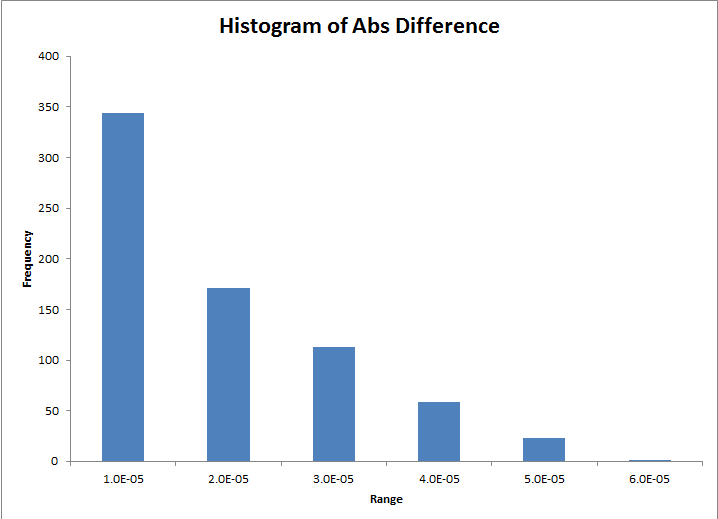
\includegraphics[width=0.8\textwidth]{118.png}
\caption{\label{fig:hist118}The histogram of the absolute differences between
measurements and estimates for the IEEE 118-bus test system .}
\label{fig:118}
\end{figure}

\begin{table} [h]
\centering
\begin{tabular}{l|r}
Properties & Values \\\hline
The number of measurements & 712 \\
Solution tolerance	& $10^{-4}$ \\
max difference	&  $6.0*10^{-5}$ 
\end{tabular}
\caption{\label{tab:118} Validation results for IEEE 118-bus test system.}
\end{table}


\newpage
\section{3000-bus test system}
\label{sec:3000}

For the 3,000-bus system, 24,105 measurements were applied to test the SE. As
shown in Figure \ref{fig:3000} , most state estimates are close to the
measurement values. The largest difference between measurements and estimates
is $8.0*10^{-5}$, smaller than the tolerance.  Table \ref{tab:3000} summarizes
the validation results.

\begin{figure}[h]
\centering
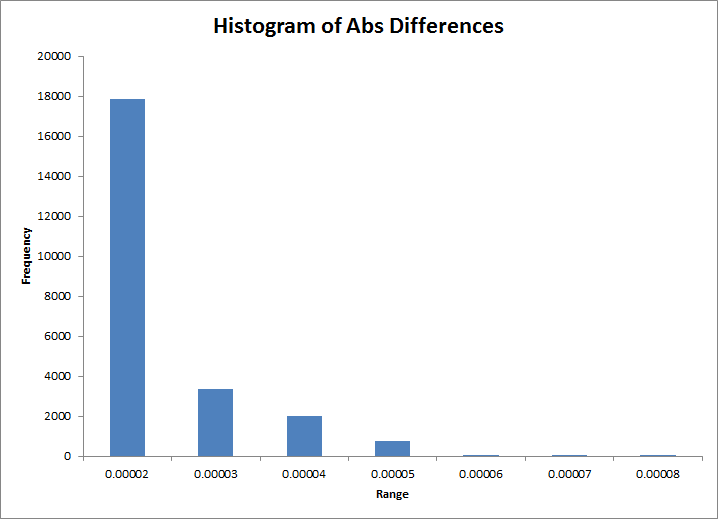
\includegraphics[width=0.8\textwidth]{3000.png}
\caption{\label{fig:hist3K}The histogram of the absolute differences between
measurements and estimates for the 3,000-bus test system .}
\label{fig:3000}
\end{figure}

\begin{table} [h]
\centering
\begin{tabular}{l|r}
Properties & Values \\\hline
The number of measurements & 24,105\\
Solution tolerance	& $10^{-4}$ \\
max difference	&  $8.0*10^{-5}$ 
\end{tabular}
\caption{\label{tab:3000} Validation results for the 3000-bus test system.}
\end{table}


\newpage
\section{20,000-bus test system}
\label{sec:20000}

The 20,000-bus system represents a western United State power grid
(WECC system). The number of measurements is 74,747. As shown in
Figure \ref{fig:20000}, the largest absolute difference between measurements
and estimates is $9.0*10^{-5}$, smaller than the tolerance. Table
\ref{tab:20000} summaries validation results.

\begin{figure}[h]
\centering
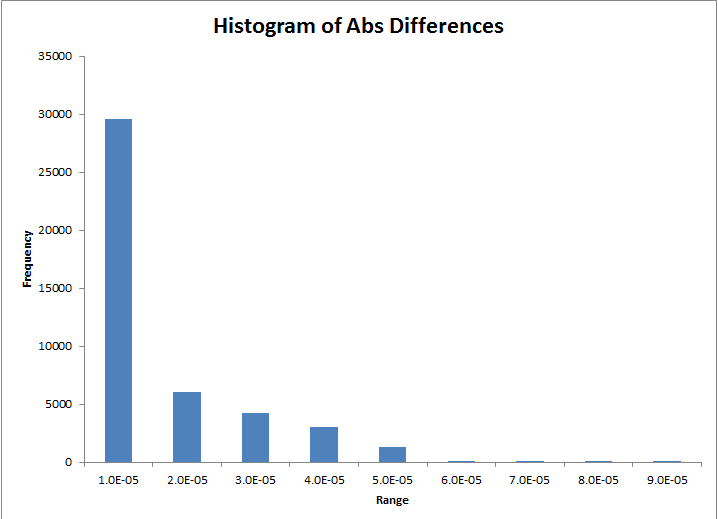
\includegraphics[width=0.8\textwidth]{20000.png}
\caption{\label{fig:hist20K}The histogram of the absolute differences between
measurements and estimates for the 20,000-bus test system.}
\label{fig:20000}
\end{figure}

\begin{table} [h]
\centering
\begin{tabular}{l|r}
Properties & Values \\\hline
The number of measurements & 74,747 \\
Solution tolerance	& $10^{-2}$ \\
max difference	&  $9.0*10^{-5}$ 
\end{tabular}
\caption{\label{tab:20000} Validation results for  the 20,000-bus test system.}
\end{table}



In summary, all the test results above have shown that GridPACK SE meets the validation requirements.

\end{document}
